\chapter{Diagramas UML}

Este capítulo presenta los diagramas UML del sistema: el diagrama de flujo de información, el diagrama de componentes, los diagramas de clases del agente (PEP) y de la API (PDP), y un diagrama de objetos con una instancia real.

\section{Diagrama de flujo de información}

\begin{figure}[h]
	\centering
	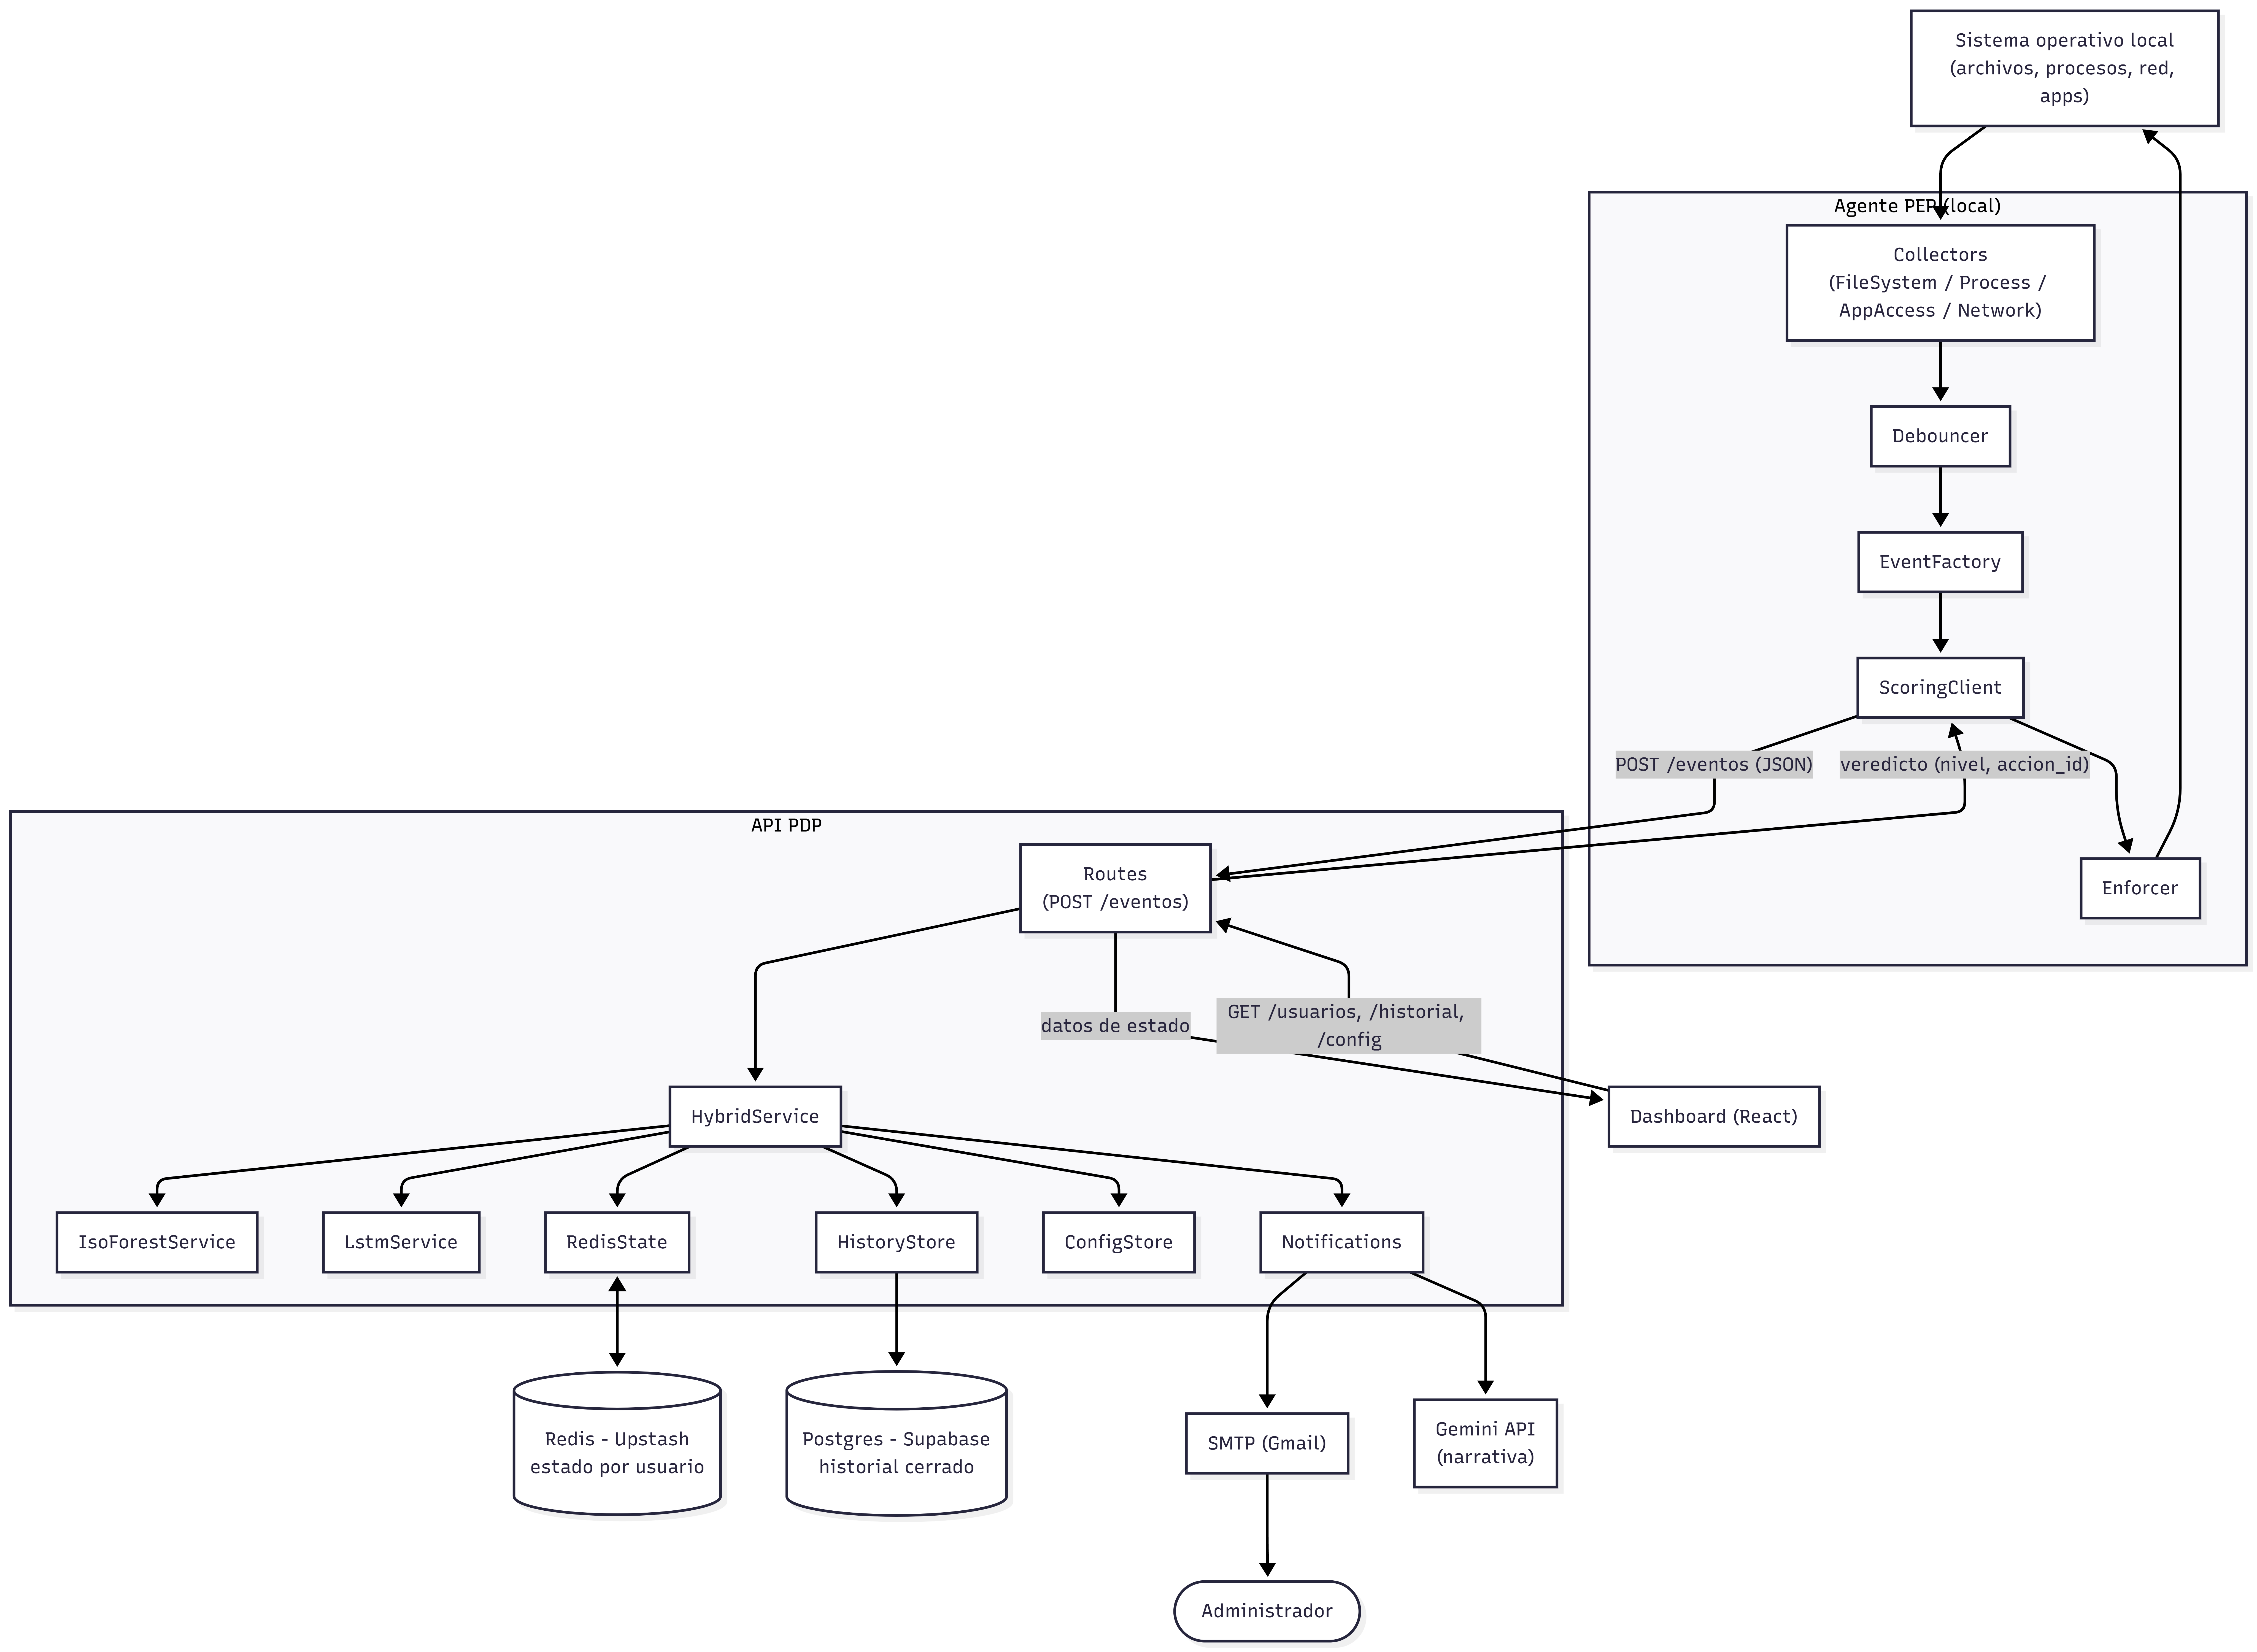
\includegraphics[width=\textwidth]{images/diagramas/diagrama-flujo.png}
	\caption{Diagrama de flujo de información del sistema.}
	\label{fig:diagrama-flujo}
\end{figure}
\FloatBarrier

\clearpage
\section{Diagrama de componentes}

\begin{figure}[h]
	\centering
	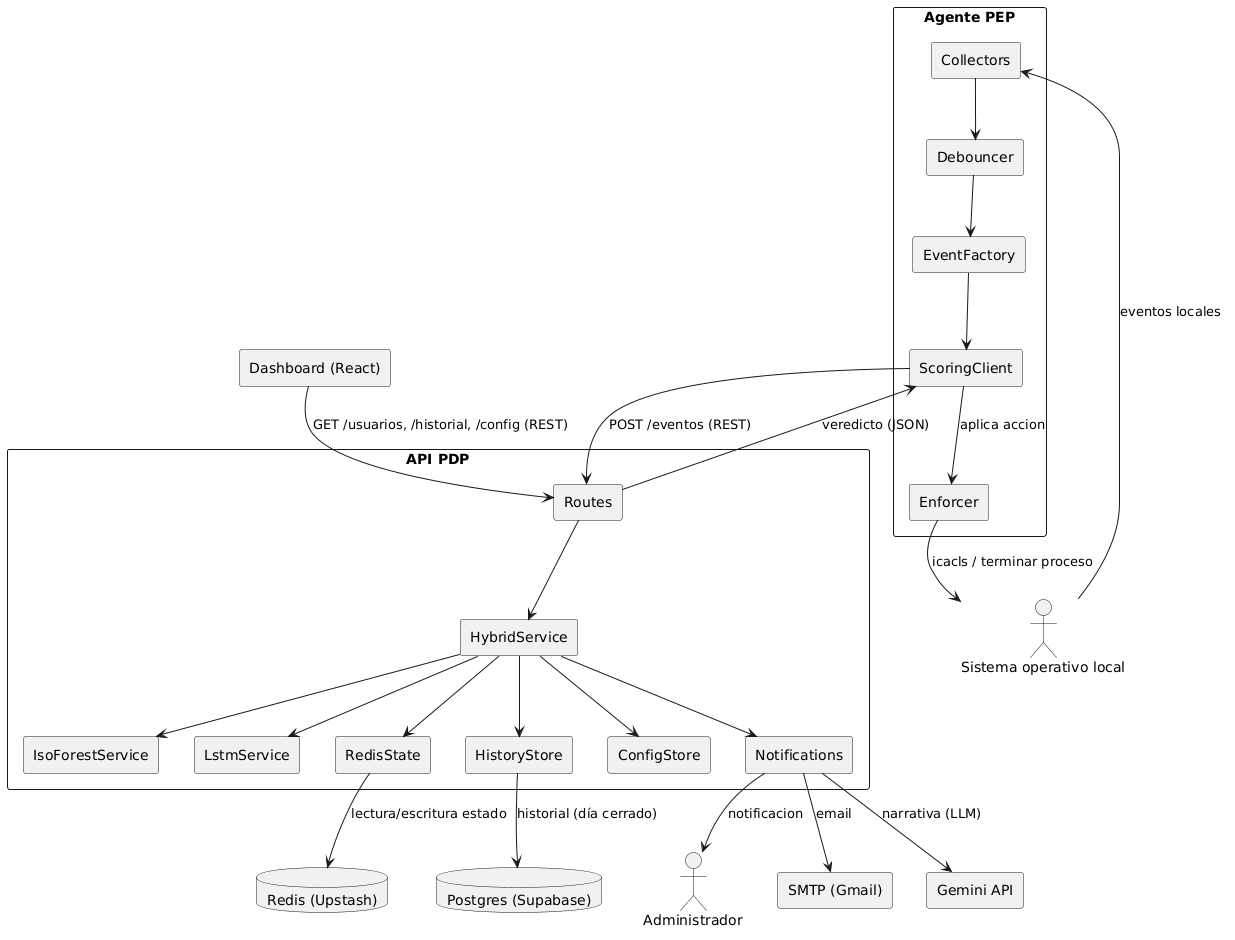
\includegraphics[width=\textwidth]{images/diagramas/diagrama-componentes.png}
	\caption{Diagrama de componentes con protocolos de comunicación.}
	\label{fig:diagrama-componentes}
\end{figure}
\FloatBarrier

\clearpage
\section{Diagrama de clases --- Agente PEP}
\begin{figure}[h]
	\centering
	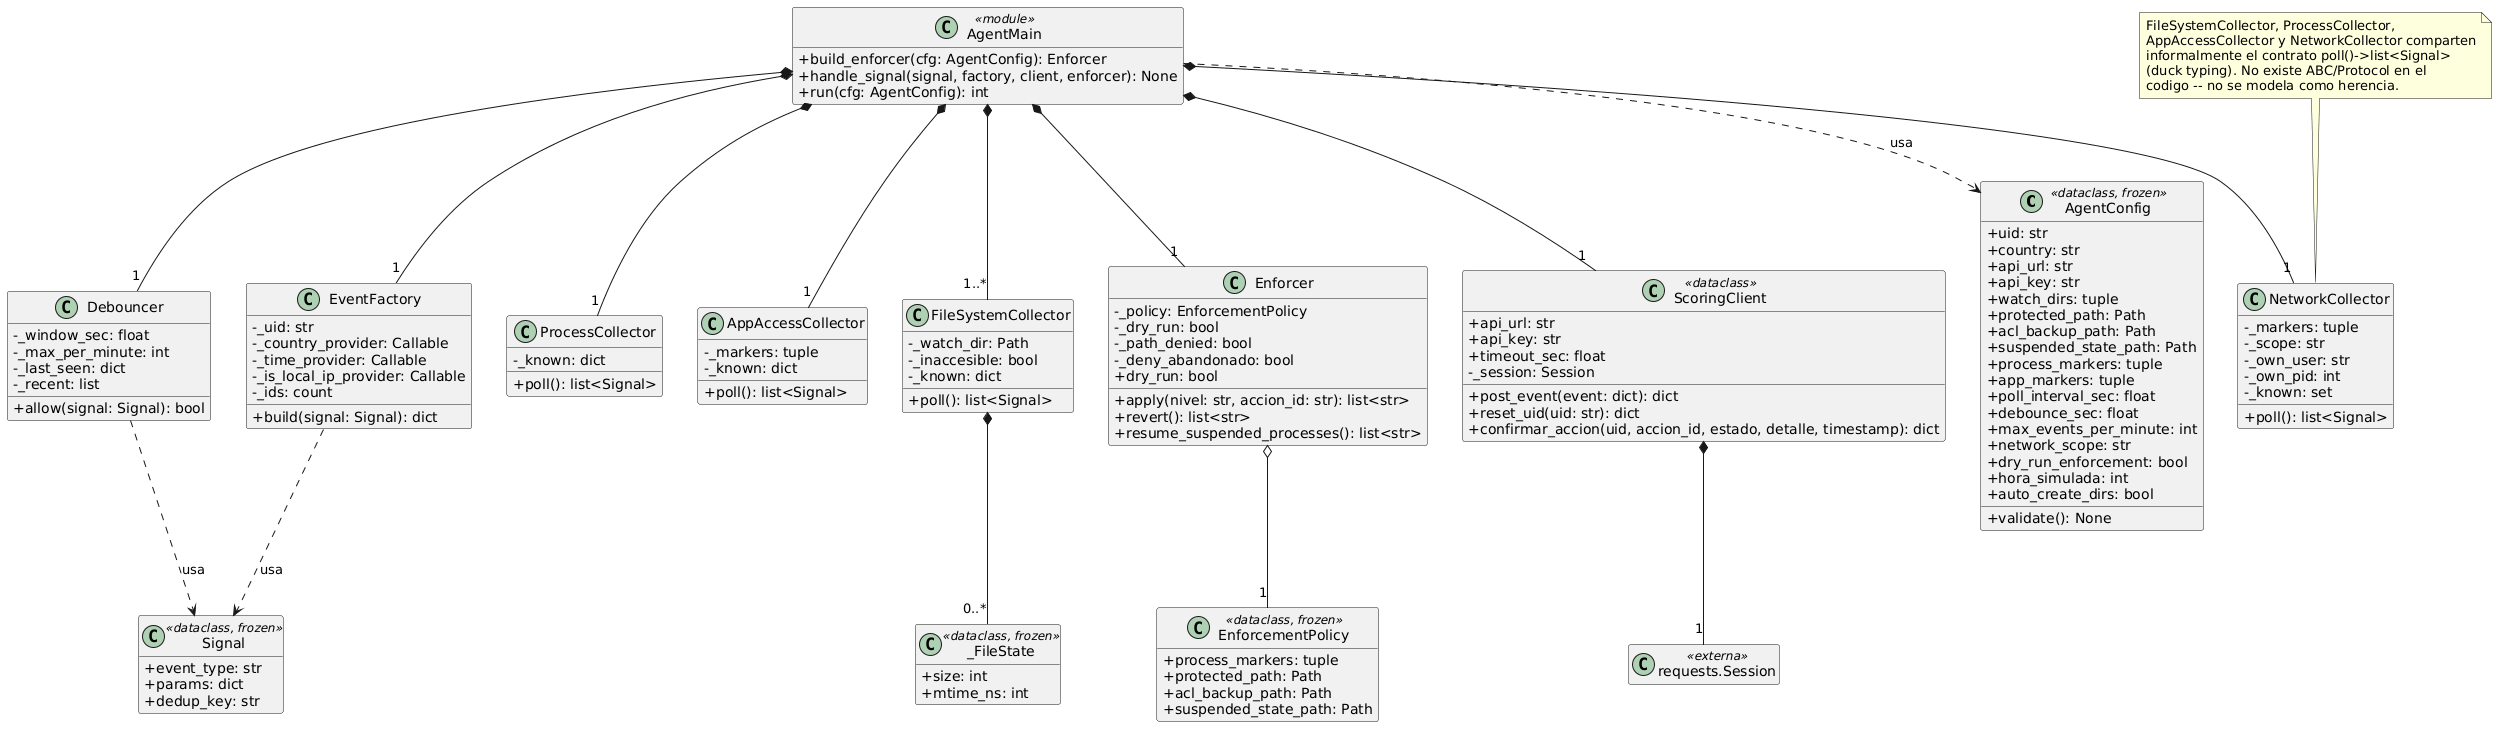
\includegraphics[width=\textwidth]{images/diagramas/diagrama-clases-agente.png}
	\caption{Diagrama de clases del Agente PEP.}
	\label{fig:diagrama-clases-agente}
\end{figure}
\FloatBarrier

\clearpage
\section{Diagrama de clases --- API PDP}
\begin{figure}[h]
	\centering
	\includegraphics[width=\textwidth]{images/diagramas/diagrama-clases-api.png}
	\caption{Diagrama de clases de la API PDP.}
	\label{fig:diagrama-clases-api}
\end{figure}
\FloatBarrier

\clearpage
\section{Diagrama de objetos}
\begin{figure}[h]
	\centering
	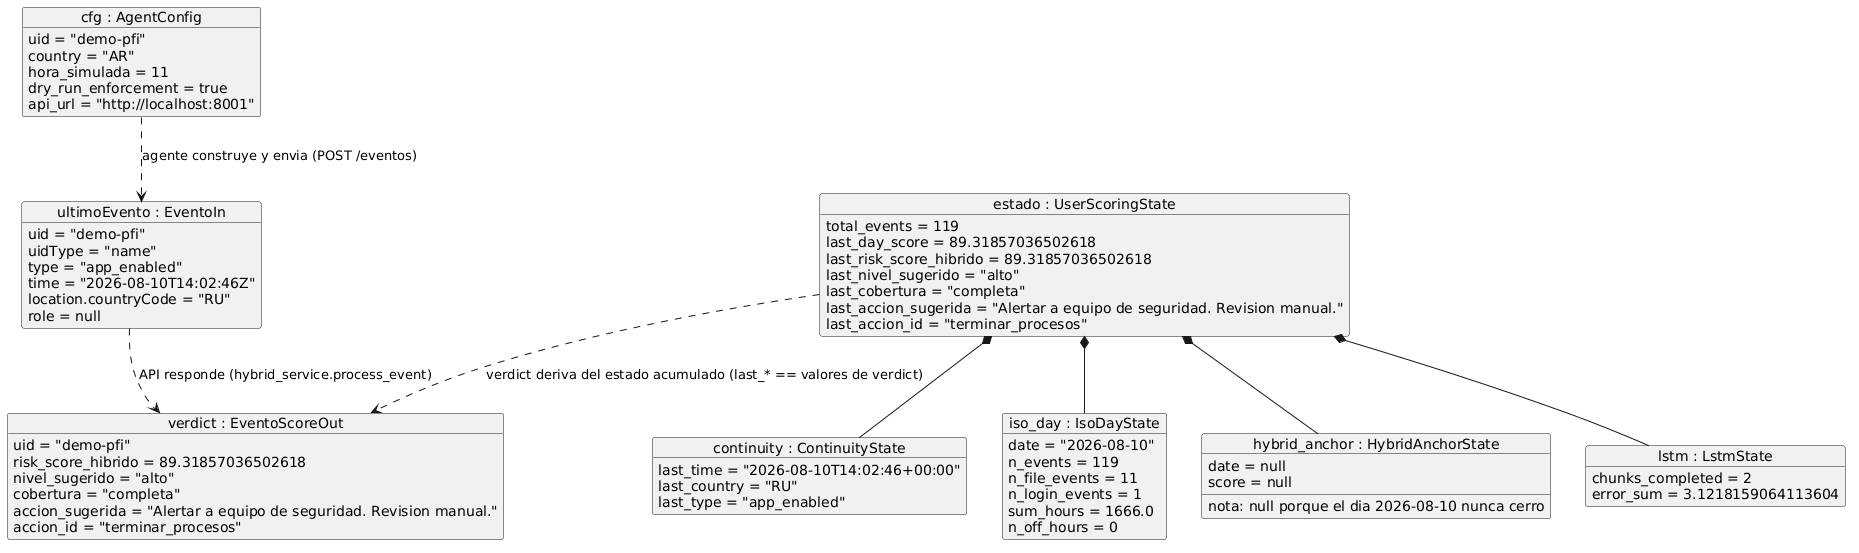
\includegraphics[width=\textwidth]{images/diagramas/diagrama-objetos.png}
	\caption{Diagrama de objetos con una instancia real (uid \texttt{demo-pfi}).}
	\label{fig:diagrama-objetos}
\end{figure}
\FloatBarrier

\clearpage
